% Proposal for the features and scoring and stuff of my senior project.
\documentclass{article}
\title{Senior Project Presentation}
\author{Steve Jarvis}
\date{\today}
% Disables chapter and section numbering
\setcounter{secnumdepth}{-1} 
\usepackage[pdftex]{graphicx}
\usepackage{listings}
\usepackage[T1]{fontenc}

\begin{document}
\maketitle

\section{What I Learned...}

\subsection{What's a Neural Network?}

    \paragraph{}A neural network is a general machine learning tool that can be 
    used to represent artificial intelligence on a wide variety of data sets. 
    A conventional artificial neural network learns by making an estimate, getting 
    feedback, and adjusting the priority given to all its connections (neurons) 
    in such a way that it inches towards the correct answer.

    \paragraph{}The simplest neural network is one consisting of two layers. A 
    weight connects each node in the first layer to each node in the second layer.
    Such a network could be trained to learn learn logical OR. Imagine three input 
    nodes and two output, with the bottom left representing false and the bottom 
    right true. When inputting bits representing logical OR, the network should 
    yield output representing true (in this case, a positive value in the right
    output node and negative in the left output node). See 
    Figure~\ref{basicnetwork} on  page~\pageref{basicnetwork} for an 
    illustration. The output will surely be wrong initially, so the error for 
    each output node is calculated, used to change the corresponding weights, 
    and continues back up the graph. The next time the network comes across 
    similar input it will give an estimate slightly closer to the desired answer.

    \paragraph{}An important consideration for this sample network is its limited 
    learning ability. A two-layer network can only learn linearly separable 
    functions; equations whose positive and negative results, when graphed, can 
    be partitioned by a single line. More complex functions require deeper networks
    to learn, although the power increases quickly. With only a single extra 
    layer (and ~200 nodes per layer) the neural net used in this project was able 
    to achieve 93 percent accuracy on the MNIST Database of Handwritten 
    Digits\footnote{For more information about the MNIST Database see
    http://yann.lecun.com/exdb/mnist/}.

    \begin{figure}
        \centering
        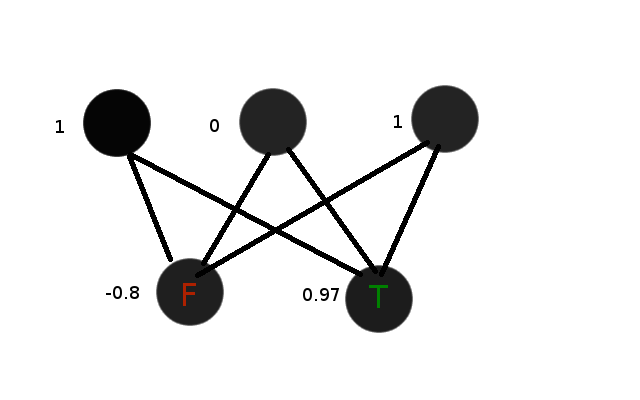
\includegraphics[scale=0.4]{images/perceptron.png}
        \caption{The top layer are inputs, connected by weights to the bottom 
            layer. The weights are changed during training so that they give the 
            desired output for the right input. A common implementation is to use 
            activation functions with a range such that -1 < y < 1, so assuming 
            the network is trained to represent true with 1 and false with -1, this 
            would be a great output.}
        \label{basicnetwork}
    \end{figure}

\subsection{Why Is There An Extra Input Node?}

    \paragraph{}The third input node is a bias. The purpose of the bias is 
    to allow any necessary shifting of the activation function. For example, the 
    activation function for the network used in this project is hyperbolic 
    tangent. It was used because it has a domain of all real numbers, it is smooth, 
    continuous, and symmetrical, and the range is -1 to 1. It is also easily 
    derived, which is important in training. During evaluation, the weights of the 
    neural network are applied as coefficients in the activation function. 
    As the weights change, the steepness of the graph is manipulated, but the 
    y-intersect is always 0 (See Figure~\ref{bias}). The bias node allows shifting
    of the entire graph, which is the only way to train something other than a 0 
    output for a 0 input. For example, without a bias node, the two layer network 
    would not be able to learn logical NAND, even though the function is linearly 
    separable.

    \begin{figure}
        \centering
        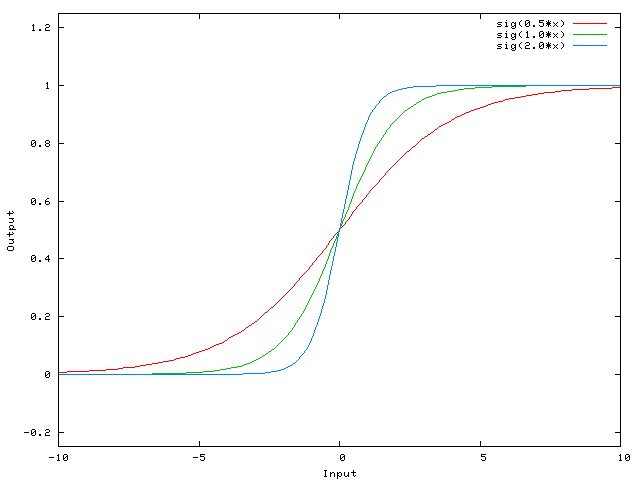
\includegraphics[scale=0.5]{images/bias.png}
        \caption{The graph of a general sigmoidal function as the coefficients 
            (weights) change. Pic taken from StackOverflow: 
            http://stackoverflow.com/questions/2480650/role-of-bias-in-neural-networks}
        \label{bias}
    \end{figure}

\subsection{How Are the Correct Weights Calculated?}

    \paragraph{}Finding the right weights is all the work. The correct weights are
    found via a process called back propagation. Back propagation is a repeated 
    process of error correction, starting with the output nodes and moving back up
    the network. The error of the output nodes is simply the difference between the
    desired output and the actual output, but the error calculation for each node 
    higher up the tree must be a summation of all collective errors of the exiting 
    connections, since each node is connected to every node in the level lower. 
    This algorithm proved to be the most difficult part of the project and I 
    consulted numerous and tutorials and open source 
    projects.\footnote{Here are some of the most helpful resources I found: \\  
    http://www.cs.montana.edu/~grayd/backprop.htm \\ 
    http://arctrix.com/nas/python/bpnn.py}
    
    \paragraph{}The network is always training in the background so the user can 
    see potentially constant improvement, and to learn more and different 
    handwriting there only needs to be more data added for the training instance 
    to reference. Also, the network takes very long to train. At the time of this 
    presentation, this network will have been training on euclid for about a 
    month, and that's not unusual. Because of the dependency on 
    adjacent layers in back propagated training, parallelization is difficult to
    implement successfully and efficiently\footnote{
    https://research.microsoft.com/apps/pubs/default.aspx?id=173312}. Parallelized
    training would be a great future endeavor but was beyond the scope of this 
    project.

    \paragraph{}Earlier it was mentioned that hyperbolic tangent is easily derived
    and that's nice for training. This is because we can use the derivative of the 
    activation function in calculating the weight deltas. Consider how the 
    derivative changes as the hyperbolic tangent is traveled. Since the derivative 
    is greatest towards the middle -- where the activation is most uncertain -- 
    results in the middle will cause a greater change in the associated weights. 
    Conversely, as the network's weights become more established through training 
    the derivative approaches zero and stabilizes the network.

\subsection{iOS, JSON, and CGI.}

    \paragraph{}I wanted a good way to demonstrate the working neural network. Just
    knowing it can recognize handwritten characters in a database is not very 
    exciting, but having it recognize a user's in real time would be. So an iOS 
    front end was created to take input, query the server on which the network is 
    running, and display the most likely results of which digit 
    was entered. The only particular I'd like to mention is how surprisingly easy 
    it was to have Apache serve Python files. A single line file in the pub 
    directory on euclid is all it takes. \\

    \begin{lstlisting}
    File: .htaccess

    AddHandler cgi-script .py
    \end{lstlisting}

\section{Software Design...}

\subsection{How It Works.}

    \paragraph{}Each image of a handwritten digit is divided into 196 logical 
    sections. The samples from the MNIST database are 28x28 pixel images, so to 
    maintain a physical square with no extraneous pixels the image had to be 
    represented with either 4, 16, 49, 196, or 784 sections\footnote{These are 
    special sizes that are both perfect squares and evenly divisible by 28.}. 
    Based on various runs of the experiment (a special mode of network training) 
    it was decided that 196 yielded the best balance of complexity and image 
    granularity. See an example of the experiment's results in 
    Figure~\ref{experiment}. In all, the production neural network has 201 inputs,
    201 hidden nodes, and 10 outputs. 196 of the inputs are a simple binary 
    representation of the presence of ink in that section. The additional five 
    inputs represent the relative distribution of ink in the image -- percent of
    ink north of the horizon, south of the horizon, west of middle, east of 
    middle, and percent of total sections containing ink. A section contains 
    ink if even a single pixel in that section is over a predetermined threshold.

    \begin{figure}
        \centering
        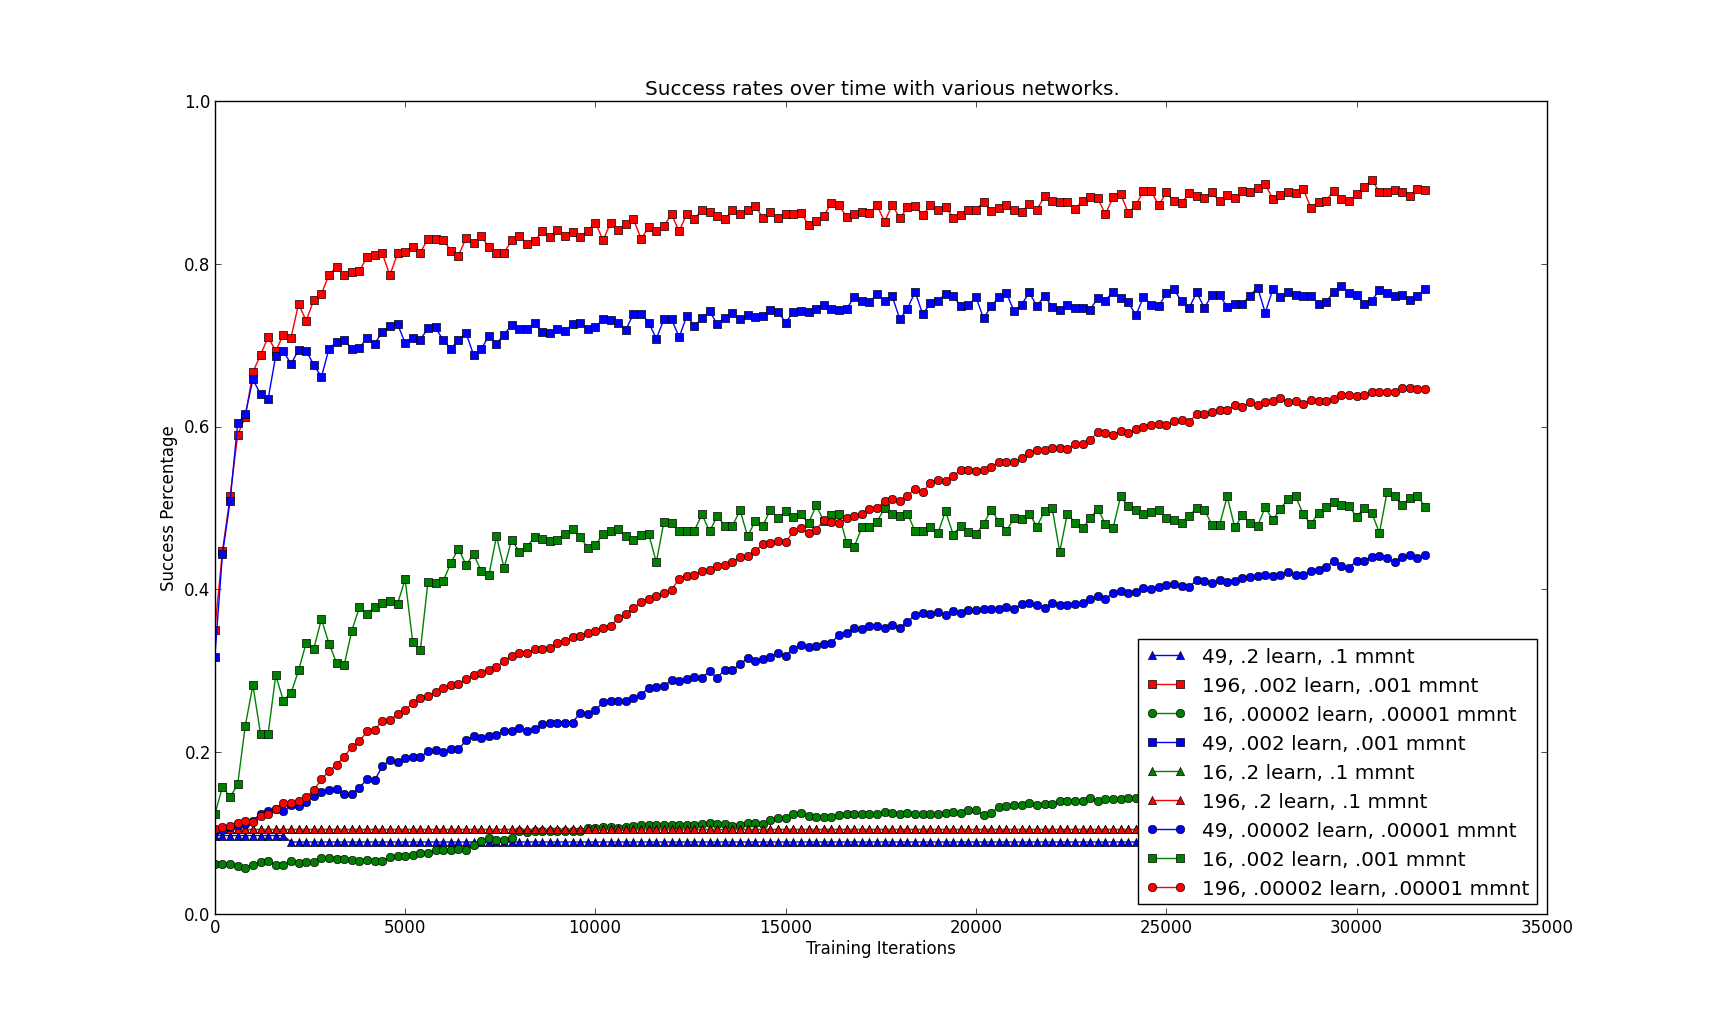
\includegraphics[scale=0.3]{images/experiment.png}
        \caption{Example output of the experiment feature of the network training
            application. Data like this helped to determine the best network 
            size and proper coefficients for learning rates. This particular run
            of the experiment took 9 hours to complete, running the experiment
            with the network for 784 section images takes multiple days to 
            complete. The key displays the network sizes (in neurons per layer) 
            and coefficients used for learning and momentum rates.}
        \label{experiment}
    \end{figure}

    \paragraph{}The same algorithms are applied to translating the MNIST data
    to network input as translating the iOS application entries to network input.
    When the user enters a digit on the iPhone application, the image is
    used to generate the binary representation described above and built into
    a web request to the web site. The site uses the neural network to interpret
    the data it receives based on the best known configuration at the time and
    outputs a JSON response of the network's estimate. The iOS application
    uses that response to display the most likely answers and associated
    certainties. See Figure~\ref{diagram} for an illustration of the interactions.
    Also note that the optimal learning and momentum rate vary
    with the complexity of the data and size of the network.

    \begin{figure}
        \centering
        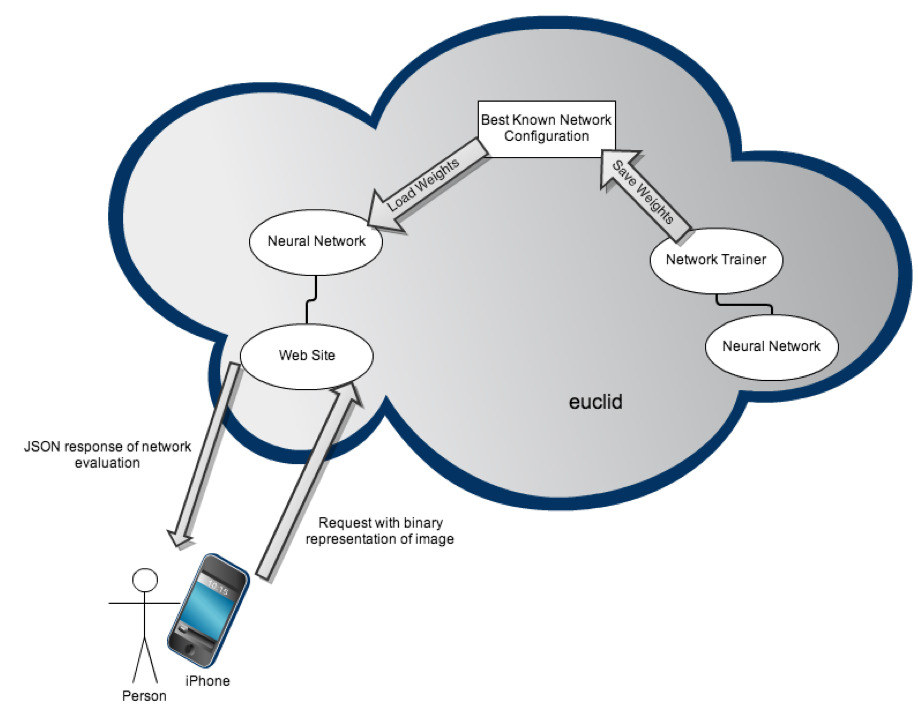
\includegraphics[scale=0.4]{images/diagram.png}
        \caption{Interaction diagram including each piece of the entire project.
            Note that the process of training, which generates the best known
            weight configurations, is entirely distinct from the user cycle 
            displayed on the left side. The only link is the sharing of the
            same weights store.}
        \label{diagram}
    \end{figure}

\subsection{How It's Organized.}

    \paragraph{}In designing this project I aimed to make it modular. Each logical
    task is the responsibility of a specific sub-application. The only exception
    is the experiment, which was used to establish near-optimal coefficients and 
    help explain unusual behavior at the start of the project.
    The experiment piggy backs as a part of the network training application 
    because of the significant overlap in funcionality. In all, there are five
    sub-applications involved in the process up to this point. The 
    live digit recognition requires the iOS application, the web site, and the
    neural network package. The training of the network, as well as the experiment,
    requires the neural network package and the network training application.

    \paragraph{}The project's parts are all under Git version control. A primary 
    goal of this project was to build a general purpose, reusable neural network, 
    so the neural network exists in a dedicated repository
    \footnote{github.com/stevejarvis/neural-network}. The other applications exist
    as subfolders of a repository created specifically for this project. The
    neural network repository is referenced as a submodule of this general 
    project repository
    \footnote{github.com/stevejarvis/scrawl-recognition}.

    \paragraph{}Since there is nothing specific to handwriting recognition in the
    network I am happy with the decision to store and reference it as an 
    indepenent package. What could use improvement is the way the network is 
    incorporated with the rest of the project. There are multiple applications 
    that rely on the neural network package yet it is added as a Git submodule 
    under the network training application's directory. It would be more 
    appropriate to have the network submodule in a more neutral location and
    reference it accordingly from the other applications. 
    
    \paragraph{}There is also substantial set up to have a completely working
    demonstration (web page, network training, adding the neural network package
    to the Python Path). It would be nice to package the applications in a way 
    that facilitates a more automated out-of-the-box solution.

\section{As Hard As I Expected...}

    \paragraph{}I was expecting really hard, and it's about what I got. There were 
    a couple especially difficult hurdles I encountered while working on this 
    project. When I first started trying to train handwritten digit recognition I 
    didn't get any performance better than about 15\% successful recognition. I 
    trained for days on even small samples of data and the success rate just 
    stalled. Worse still, it was unpredictable and inconsistent. I added an extra
    test that graphed performance as the network was scaled. I could see 
    that ``skinny" three-layer networks -- networks with fewer than about 60 nodes 
    per layer -- mastered data sets quickly and flawlessly. As the networks grew 
    larger they became wildly inconsistent. The test trained a constant 
    function for a constant number of iterations on increasingly large networks and 
    graphed the error rate and time to completion versus size. Figure~\ref{badgraph}
    shows the initial results. There were so many moving pieces I couldn't imagine 
    what the issue was. It turns out the answer was local minima, and that turning the 
    learning and momentum rates down significantly would help to avoid sticking points.
    Figure~\ref{goodgraph} shows the nearly flawless performance of the improved 
    network.

    \paragraph{}The next great challenge was improving the disappointingly poor 
    performance of real life digit recognition. The network was training on euclid 
    as I was finishing the basic functionality of the iOS application, and by the 
    time I finished the logs read it was correctly recognizing more than 93\% of 
    the test data. In actual use, however, I found the network to correctly 
    interpret only the nicest of input; perfectly sized and centered submissions.
    The problem was the strict preprocessing done on the data in the MNIST Database
    did not accurately represent unfiltered data from the real world. To improve 
    performance, I ``messied" up the training data by adding variations on size 
    and rotation. The samples I added turned the training set of ~40k samples 
    into a set of ~1.5M samples. 

    \paragraph{}Shortly after adding the new data I learned the three layer 
    network was unable to learn it, it introduced too much complexity.
    To overcome this I added a fourth layer of neurons.
    Similar to the bump from two to three layers, the change from three to four 
    meant lower learning rates to avoid the increased chance of becoming stuck in 
    local minima and longer training times to facilitate the exponentially 
    increased number of connections. 
    
    \paragraph{}Now, finally, it seems to be working with acceptable
    performance. To further increase the success I believe finding an 
    appropriate bounding box before sending data from the iOS 
    application would give noticeable improvements.

    \begin{figure}
        \centering
        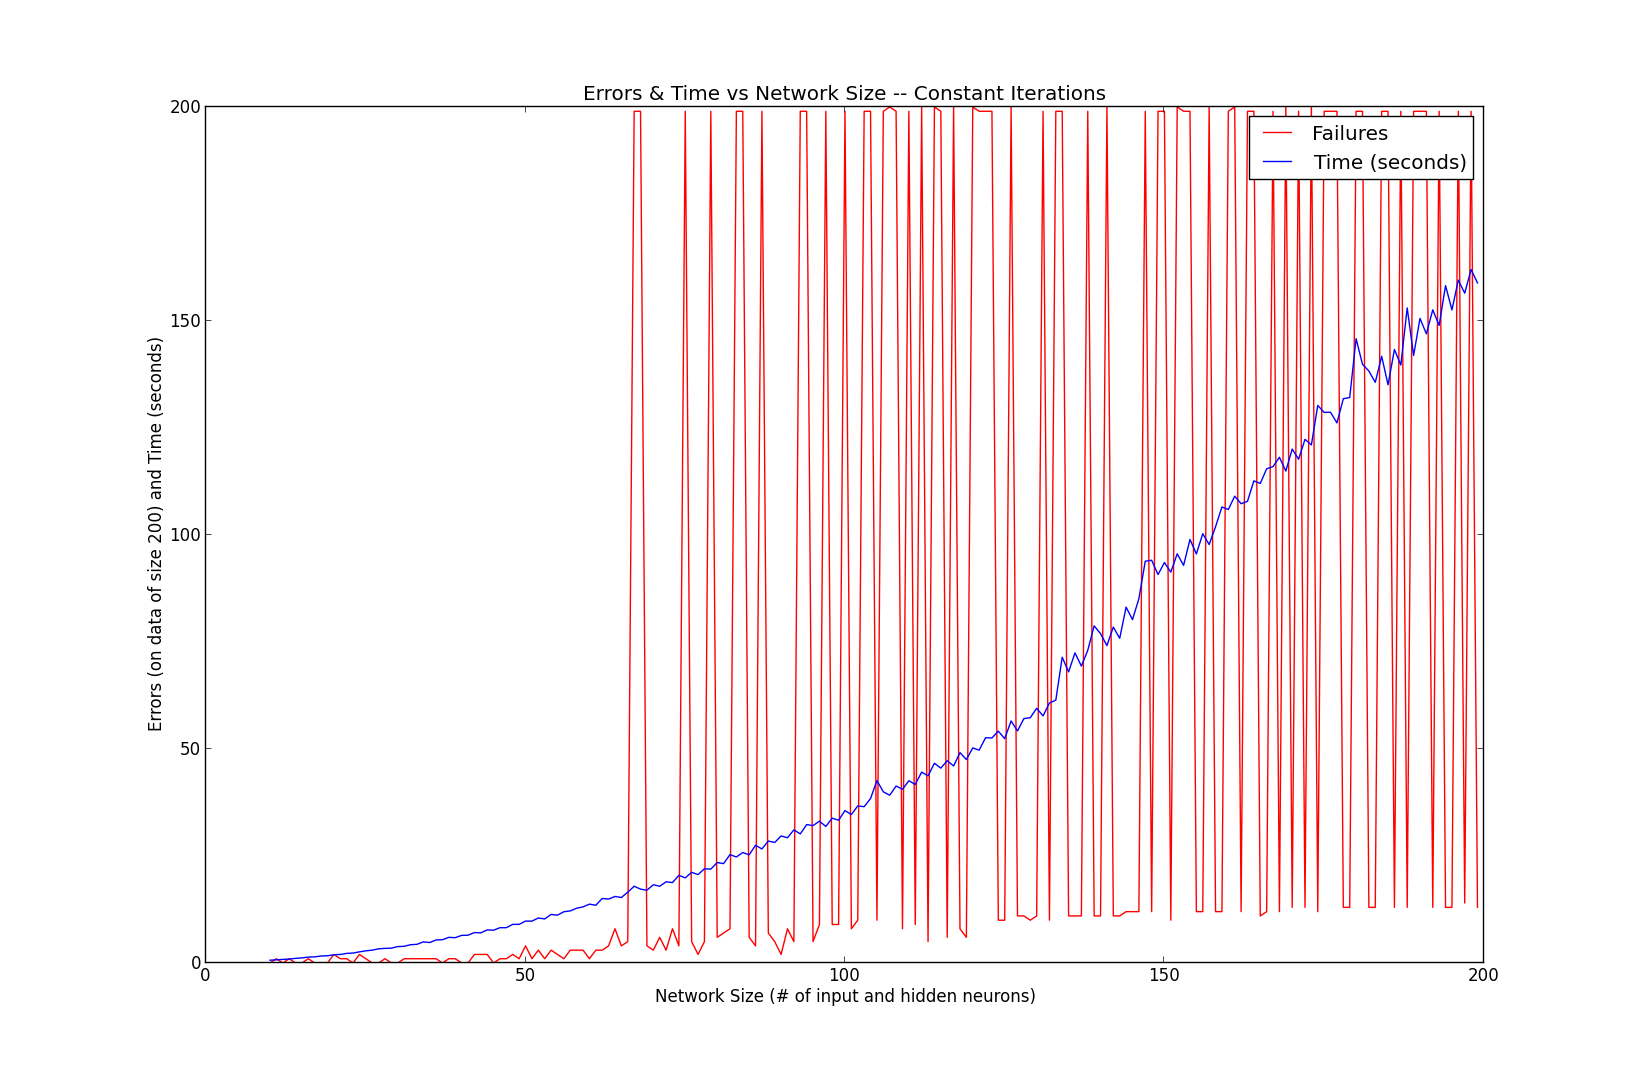
\includegraphics[scale=0.3]{images/bad_learning.png}
        \caption{Early scaling test run with bad learning rates. Notice that
            as the network grows larger the success of the network becomes as
            unsure as a coin flip.}
        \label{badgraph}
    \end{figure}

    \begin{figure}
        \centering
        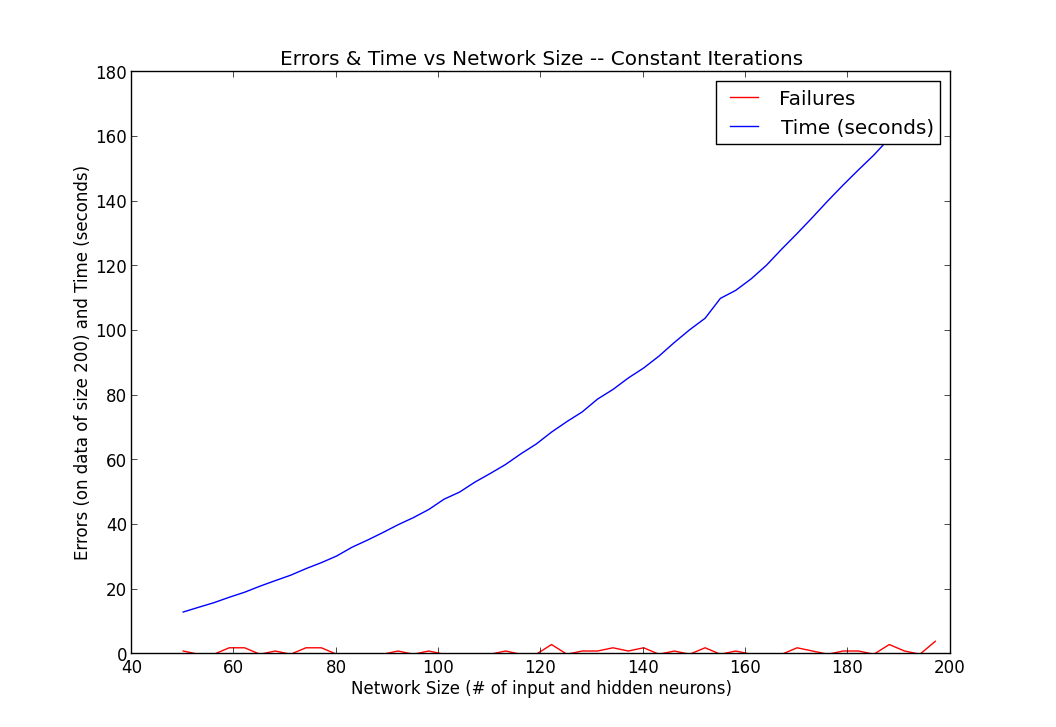
\includegraphics[scale=0.5]{images/good_learning.png}
        \caption{The scaling test run with a learning rate and momentum rate 
            1/1000th of the magnitudes used in Figure~\ref{badgraph}}
        \label{goodgraph}
    \end{figure}

    \paragraph{}Here are the approximate line 
    counts\footnote{Found by wc. iOS App is forked from GLPaint by Apple: 
    https://developer.apple.com/library/ios/\#samplecode/GLPaint/}. \\

    \begin{tabular}{ l c r }
        Part & Line Count & Language \\
        \hline \\
        Neural Network & 542 & Python \\
        Network Training & 1142 & Python \\
        Web Site & 67 & Python \\
        iOS App & 1564 & Objective C \\
        Total & 3315 & All \\
    \end{tabular}

\end{document}
